\documentclass[zihao=-4]{ctexart}
\usepackage[normalem]{ulem}
\useunder{\uline}{\ul}{}
%********************导言区宏包引入********************
\usepackage{xeCJK}
\usepackage{gbt7714}
\usepackage{amssymb}
\usepackage{amsmath}
\usepackage{listings} %代码
\usepackage{graphicx}
\usepackage{multicol} %回车换段
\usepackage{xcolor}
\usepackage{geometry} %页面设置
\usepackage{fontspec}
\usepackage{setspace}
\usepackage{times}
\usepackage{fancyhdr} %页眉页脚
\pagestyle{fancy}
\usepackage{float} %表格位置
\usepackage{titlesec} %设置
\usepackage{titletoc}
\usepackage{ctex}
\usepackage{gbt7714}    %控制参考文献格式为国标
\usepackage{multirow}
\usepackage{booktabs}   %表格相关
\usepackage{setspace}   %设置行距
\usepackage{caption} %caption
\usepackage{subcaption} %子图的caption
\usepackage{changepage} %左右缩进
\usepackage{makecell}


\graphicspath{ {include_picture/} }
\let\algorithm\relax
\let\endalgorithm\relax
\usepackage[ruled,vlined]{algorithm2e}%[ruled,vlined]{
\usepackage{algpseudocode}
\renewcommand{\algorithmicrequire}{\textbf{Input:}} 
\renewcommand{\algorithmicensure}{\textbf{Output:}}
%\renewcommand\thepage{\zihao{-5} ~\arabic{page}~}%页码字号

%定义两个arg
\DeclareMathOperator*{\argmax}{arg\,max}
\DeclareMathOperator*{\argmin}{arg\,min}
\DeclareCaptionLabelSeparator{mysep}{\space\space}  %自定义caption格式
\captionsetup[figure]{font={small}, labelfont=bf, labelsep=mysep, textfont=bf}   %图片caption格式
\captionsetup[table]{font={small}, labelfont=bf, labelsep=mysep, textfont={bf}}   %表格caption格式
\bibliographystyle{gbt7714-numerical} %修改了title斜体内容

%********************导言区宏包引入********************
%********************第三方字体引入********************
%\setCJKmainfont[Path=fonts/,BoldFont=simhei.ttf,ItalicFont=simkai.ttf,SlantedFont=simfang.ttf]{simsun.ttc}
%中文字体涵盖黑体、宋体、楷体、仿宋
\setmainfont[Path=fonts/, 
BoldFont = times-new-roman-bold.ttf,
ItalicFont = times-new-roman-italic.ttf,
BoldItalicFont = times-new-roman-bold-italic.ttf
]{times-new-roman.ttf}
\setmonofont[Path=fonts/]{Courier New.ttf}
\setCJKfamilyfont{hwzs}[Path=fonts/]{STKzhongsong.ttf}%使用STZhogsong华文中宋字体
\newcommand{\zhongsong}{\CJKfamily{hwzs}}
\setCJKfamilyfont{hwxw}[Path=fonts/]{STKxinwei.ttf} % XSP 2023/3/3:
\newcommand{\xinwei}{\CJKfamily{hwxw}}              %  使用STZxinwei华文新魏字体.

%********************第三方字体引入********************


%********************中文字号设置********************
%\newcommand{\chuhao}{\fontsize{42pt}{\baselineskip}\selectfont}
\newcommand{\chuhao}{\fontsize{42pt}{0}}
\newcommand{\xiaochu}{\fontsize{36pt}{0}}
\newcommand{\yihao}{\fontsize{28pt}{0}}
\newcommand{\erhao}{\fontsize{21pt}{0}}
\newcommand{\xiaoer}{\fontsize{18pt}{0}}
\newcommand{\sanhao}{\fontsize{16pt}{0}}
\newcommand{\sihao}{\fontsize{14pt}{0}}
\newcommand{\xiaosi}{\fontsize{12pt}{0}}
\newcommand{\wuhao}{\fontsize{10.5pt}{0}}
\newcommand{\xiaowu}{\fontsize{9pt}{0}}
\newcommand{\liuhao}{\fontsize{8pt}{0}}
\newcommand{\qihao}{\fontsize{5.25pt}{0}}
%********************中文字号设置********************


%********************页边距设置********************
\geometry{left=3cm,right=2cm,top=2.5cm,bottom=2.5cm}
\geometry{a4paper} % xsp 2023/3/7: 调整纸张大小为A4
%********************页边距设置********************

%********************段间距设置********************
\newcommand{\setParDis}{\setlength {\parskip} {0pt} }
%请在每部分使用这个
%********************段间距设置********************
%********************

\begin{document}
%********************页眉页脚设置********************
\lhead{}%设置左页眉为空
\rhead{}%设置左页眉为空
\setlength{\headwidth}{\textwidth}% 2023/3/3 XSP: 页眉长度适应文本
%********************页眉页脚设置********************


%********************标题格式设置********************

%\setcounter{secnumdepth}{0}%该命令取消了章标题前数字label

\CTEXsetup[name={,、},number={\chinese{section}}]{section}
\CTEXsetup[name={(,)},number={\chinese{subsection}}]{subsection}
\CTEXsetup[name={,.},number={\arabic{subsubsection}}]{subsubsection}% 不加会导致目录格式错误
% 设置subsubsection等格式
% \titleformat{\section}[block]{\sanhao\bfseries\centering}{\chinese{section}、}{0pt}{}[]
% \titleformat{\subsection}[block]{\sihao\bfseries}{(\chinese{subsection})}{0pt}{}[]
% \titleformat{\subsubsection}[block]{\xiaosi\bfseries}{\arabic{subsubsection}、}{0pt}{}[]
\titleformat{\section}[block]{\sanhao\heiti\centering}{\chinese{section}、}{0pt}{}[]    % XSP 2023/3/3:
\titleformat{\subsection}[block]{\sihao\heiti}{(\chinese{subsection})}{0pt}{}[]       %   将正文标题字体由加粗
\titleformat{\subsubsection}[block]{\xiaosi\heiti}{\arabic{subsubsection}.}{0pt}{}[]   % 修改为黑体。
\titlespacing{\section}{0pt}{25pt}{12pt}
\titlespacing{\subsection}{0pt}{7pt}{7pt}
\titlespacing{\subsubsection}{0pt}{5pt}{4pt}

\titlecontents{section}[1.6em]{\addvspace{2pt}\filright}
{\contentspush{\thecontentslabel\hspace{0.8em}}}
{}{\titlerule*[8pt]{.}\contentspage}

\titlecontents{subsection}[3.2em]{\addvspace{2pt}\filright}
{\contentspush{\thecontentslabel\hspace{0.8em}}}
{}{\titlerule*[8pt]{.}\contentspage}

\titlecontents{subsubsection}[6.4em]{\addvspace{2pt}\filright}
{\contentspush{\thecontentslabel\hspace{0.8em}}}
{}{\titlerule*[8pt]{.}\contentspage}
%********************标题格式设置********************

%\setcounter{section}{-3}  %标题计数器
%\stepcounter{section}

%*******************行间距段前段后*******************
\linespread{1.8}
%行间距为实际行间距乘以1.2,如此处实际为1.5倍行距
\setlength{\parskip}{0.5\baselineskip}
%*******************行间距段前段后*******************


%********************封面部分********************
%
%     论文题目:应准确、鲜明、简洁,能概括整个论文中最主要和最重要的内容。
% 题目不超过20个中文字,若语意未尽,可用副标题补充说明。副标题应处于从属
% 地位,一般可在题目的下一行用破折号“——”引出。论文题目应避免使用不常用缩
% 略词、首字母缩写字、字符、代号和公式等。
%
\def\Fengru{第三十四届“冯如杯”竞赛创意赛道}
\leftline{
\includegraphics[scale=1]{include_picture/xiaohui.png}} % XSP 2023/3/3: 取消校徽段首缩进
%格式控制部分
% \par \  
% \par \
% \par \
\vspace{32pt}
\begin{center}

\includegraphics[height=2.25cm, width=12.78cm, scale=1]{include_picture/xiaoming.png}
\end{center}
%格式控制部分
\vspace{12pt}

\begin{spacing}{3}
    % \erhao
    \begin{center}
      {
        \fontsize{22pt}{3}\selectfont
        \zhongsong{基于检索增强生成的协作与资源管理系统设想} %黑体这样调用,其余字体同理
      } 
        % \zhongsong{“冯如杯”竞赛主赛道项目是什么}
    \end{center}
    \rightline{\xinwei\sanhao{——应用AI协助科研创新合作与资源利用最大化}} % XSP 2023/3/3: 副标题二号华文新魏居右
\end{spacing}
%格式控制部分
% \par \ 
% \par \
\par \ 
\par \
\par \ 
\par \
% \begin{center}
%     \sihao
%     \textbf{学院:计算机学院}
%     \par \ 
%     \textbf{本模板原作者:Someday}
% \end{center}

%格式控制部分
\par \ 
\begin{center}
\sanhao
\centerline{\heiti{}}%封面年月去掉
\end{center}

\pagenumbering{gobble} %封面无页码
%\thispagestyle{empty}

\renewcommand{\headrulewidth}{0pt}%没有页眉装饰线
\renewcommand{\listfigurename}{图目录}
\renewcommand{\listtablename}{表目录}
\clearpage
\pagenumbering{roman} %摘要目录页小写罗马
\xiaosi
\section*{摘要}% section*生成无标号章节
\addcontentsline{toc}{section}{摘要}
\begin{spacing}{1.5}
  \setParDis %设置段间距为 0
本文提出了一种基于检索增强生成的协作与资源管理系统,旨在解决小型科研创新团队在协同作业中的资源浪费与沟通难题。该系统将检索增强生成模型与资产管理系统相结合,通过信息检索与文本生成,优化资源配置,提高协同作业效率。

本文先介绍了该系统所使用的检索增强生成模型。检索增强生成模型具有知识自动选取和更新、保护隐私数据、降低生成成本以及跨模态和任务应用等特性,能够协助大语言模型进行长期的知识和生成内容更新与转换,避免泄露私有数据,降低计算成本,并在各种模态和任务中得到了广泛应用。

其次,本文介绍了本系统在设想中的具体构造,其包括交流平台、共享资源库和记录系统,通过检索增强生成模型实现相互连接。该系统具有技术可行性,其实际应用价值能够为小型科研创新团队协作提供新的解决方案。同时,系统还借鉴了企业人力协作系统的经验,通过使用有效的人力资源整合和利用模型,能够帮助小型团队实现高效的资源共享和合作,进而确保了其设计的合理性。

总的来说,本文提出的基于大语言模型的RAG协作与资源管理系统是一种创新性的解决方案,能够解决协同作业中的资源浪费与沟通难题,提高团队协作效率和质量。该系统具有广阔的应用前景,有望为数字时代中科研创新的发展带来新的推动力。

\end{spacing}
    
  \textbf{关键词:}大语言模型,检索增强生成,资产管理,团队协作

\newpage
\section*{\textbf{Abstract}}% section*生成无标号章节
\addcontentsline{toc}{section}{Abstract}
\begin{spacing}{1.5}
\begin{adjustwidth}{0.42cm}{0.42cm}
  \setParDis %设置段间距为 0
This article proposes a collaborative and resource management system based on retrieval-augmented generation, aimed at addressing the issues of resource waste and communication challenges in the collaborative work of small scientific research and innovation teams. By integrating the retrieval-augmented generation model with the asset management system, this system optimizes resource allocation and improves collaborative work efficiency through information retrieval and text generation.

Firstly, this article introduces the retrieval-augmented generation model used in the system. This model is characterized by automatic knowledge selection and updating, protection of private data, reduction of generation costs, and cross-modal and task applications. It can assist large language models in long-term knowledge and content updating and transformation, prevent the leakage of private data, reduce computational costs, and has been widely used in various modalities and tasks.

Secondly, this article presents the envisioned specific construction of the system, which includes a communication platform, a shared resource library, and a recording system, interconnected through the retrieval-augmented generation model. The system is technically feasible and has practical application value, providing a new solution for collaboration in small scientific research and innovation teams. At the same time, the system also draws on the experience of enterprise human resource collaboration systems. By using an effective model for integrating and utilizing human resources, it can help small teams achieve efficient resource sharing and collaboration, ensuring the rationality of its design.

Overall, the RAG collaborative and resource management system proposed in this article, based on large language models, is an innovative solution that can address the issues of resource waste and communication challenges in collaborative work, improving team collaboration efficiency and quality. This system has broad application prospects and is expected to bring new impetus to the development of the scientific research and innovation in the digital era.
\qquad 

\textbf{Keywords:} Large Language Model, Retrieval-Augmented Generation, Asset Management, Team Co-operation
\end{adjustwidth}
\end{spacing}



%********************摘要部分********************


%********************目录部分********************
\clearpage
\tableofcontents
\clearpage
%********************图表目录部分********************
\listoffigures
\listoftables

\clearpage
\renewcommand{\headrulewidth}{0.4pt} %恢复页眉装饰线

%********************正文页眉部分********************
%\lhead{} 
\chead{\xiaowu 北京航空航天大学\Fengru 参赛作品} %设置居中页眉
%********************正文页眉部分********************

\pagenumbering{arabic} %正文页码从1开始,用阿拉伯数字
\setcounter{page}{1} 

\section*{引言}% section*生成无标号章节
\addcontentsline{toc}{section}{引言}
\setParDis %设置段间距为 0
\begin{spacing}{1.5}
\subsection {应用背景}
  在如今网络极为发达的时代,我们可以较为方便地利用网络获取几乎任何所需物品和信息。然而,在与他人协同作业时,各方交流的不及时、不通畅和对各方已有资源的不熟悉等问题都可能导致信息与物品的重复获取,这一方面可能造成资源的利用率和回报率下降,另一方面也可能导致劳动力的损失。除此之外,小组各成员之间时间难以协调、空间相隔距离远、目标及资源掌握状况不同等问题也进一步造成了沟通上可能存在的障碍。

过去的几年见证了大语言模型的飞速发展,如今,多种多样的大语言模型已经得到了广泛的应用。在人机交互和信息获取方面,相较于传统搜索引擎和信息管理系统,大语言模型的优势极为显著。我们是否能够利用大语言模型的这些特性,处理协同作业时可能存在的资源浪费与沟通困难的问题呢?
\subsection {基本思路}
  目前,在我国数字经济规模在国内生产总值(GDP)中所占比例连年高升的背景下,数字化经济的发展成为必然,企业也逐步开始对资产进行数字化管理,以满足当前实际发展的需求\cite{1}。只有提高管理的能力、运用信息化软件进行管理,才能提高固定资产的管理效率\cite{2}。在企业的数字化管理进程中,部分企业所采用的智能企业资产管理(enterprise asset management, EAM)系统具有提高资产管理效率和优化资产配置、减少资源浪费等效果。倘若能将该系统套用于协同作业之上,势必能较为有效地改善上述在协同作业中可能存在的问题。

但是,对于个人用户和规模较小的科研团队而言,使用智能企业资产管理系统的成本过高,并且由于该系统主要针对于资产密集型企业而开发,也存在功能不够专门、设置操作过于复杂等问题。

基于目前市面上尚无针对于个人和小规模专门化的科研创新团队服务的现状,笔者从企业资产管理系统、新时代团队协作要点和大语言模型获得启发,将检索增强生成(Retrieval-Augmented Generation, RAG)模型与RAM系统融合,设想了本基于检索增强生成的协作与资源管理系统。


\section{检索增强生成介绍}


  顾名思义,检索增强生成的核心思想就是信息的检索与文本的生成,通过检索得到的文档来辅助生成完整的语言序列。
\subsection{检索增强生成模型的构造及原理}
  RAG模型通过使用输入序列x来检索文本文档z,并在生成目标序列y时将输入序列用作附加上下文。其主要由检索器$\mathrm{p_{\eta}(z|x)}$和生成器$p_{\theta }(y_{i}|x,z,y_{1:i-1})$两部分组成,具体运行结构及流程如下图1所示。
\begin{figure}[H] %H为当前位置,!htb为忽略美学标准,htbp为浮动图形
    \centering %图片居中
    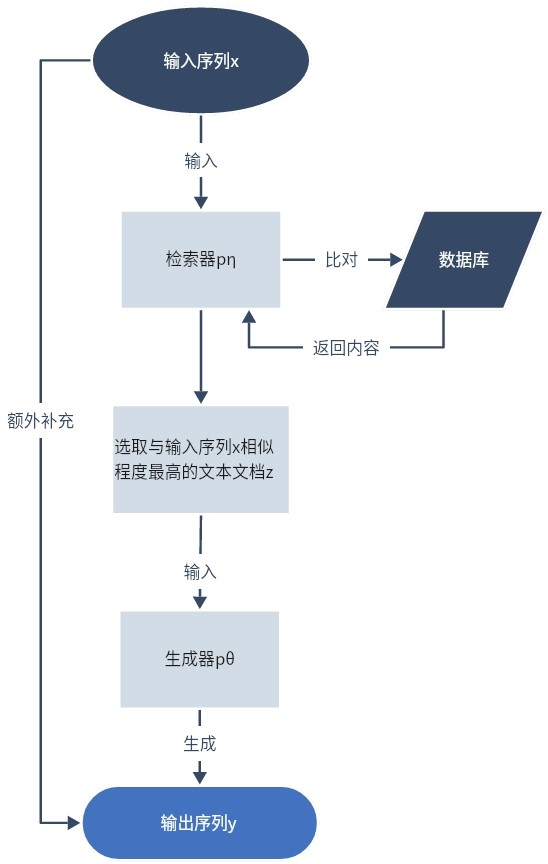
\includegraphics[width=0.6\textwidth]{RAG模型原理.jpg} %插入图片,[]中设置图片大小,{}中是图片文件名
    \caption{RAG模型构造} %最终文档中希望显示的图片标题
    \label{RAGmodel} %用于文内引用的标签
\end{figure}
\subsubsection{RAG模型}
  目前,广泛应用的RAG模型主要分为Sequence型和Token型。

\textbf{RAG-Sequence模型 }  本模型使用同一个检索文档来生成完整的输出序列。总的来说,它将检索到的文档视为一个潜在变量,通过top-K近似获得概率p(y|x)进而进行输出。更具体地讲,RAG-Sequence模型使用检索器检索前K个文档(k的值取决于检索器的设置),而生成器据此生成每个文档的输出序列概率,然后将其边缘化。其数学原理如(1)式所示,其中$\mathrm{z\in top-K(p(\cdot |x))} $。
\begin{align}
{\Huge p_{RAG-Sequence} (y|x)\approx\sum(z|x)p_{\theta } (y|x, z)  =  \sum p_{\eta }  (z|x)\prod_{i}^{N} p_{\theta }  (y_{i} |x, z,y_{1:i-1} )  } 
\label{eq1}
\end{align}

\textbf{RAG-Token模型 }  在RAG-Token模型中,我们可以为每个目标token绘制不同的潜在文档并相应地边缘化。这允许生成器在生成答案时从多个文档中选择内容。具体来说,使用检索器检索前K个文档,然后生成器为每个文档生成下一个输出令牌的分布,然后将其边缘化,并使用如(2)式所示的输出令牌重复此过程。
\begin{align}
{\Huge p_{RAG-Token}(y|x)\approx \prod_{i}^{N} \sum p_{\eta}(z|x)p_{\theta }(y_{i}|x,z,y_{1:i-1})}
\end{align}
\label{eq2}
我们已经知道,当我们将目标类视为长度为1的目标序列来用于序列分类任务时,这两种模型是等效的\cite{3}。
\subsubsection{检索器}
  检索器组件基于密集段落检索器\cite{4}(dense passage retriever, DPR)开发。给定一个M个文本段落的集合,DPR能够在低维和连续的空间中索引所有该集合中的段落,以便在运行时为读者高效地检索与输入问题相关的前k个段落\cite{4}。
\subsubsection{生成器}
  对于RAG模型而言,生成器可以使用任何编码器-解码器来建模\cite{3},即能使用任一大语言模型进行自然语言的生成。由于大语言模型原理较为复杂,且并非本文重点,在笔者能力与时间有限的情况下,不在此赘述。

  简而言之,RAG模型就是具有自动检索功能的大语言模型。RAG的自动检索这一特性使得大语言模型生成的内容更加准确的同时,能够根据应用场景的不同变得更具有针对性和个性化。
\subsection{检索增强生成的优势}
 \subsubsection{知识选取和更新 }  由于RAG模型具有能够进行数据库的热插拔的特性,因此当存在多个数据库或数据库能够及时更新,RAG便将能够协助大语言模型进行知识和生成内容的长期更新与转换。

 \subsubsection{保护隐私数据 }  RAG模型本身的检索机制使大语言模型能够根据本地库生成内容而无需将其上载,因而能够避免在生成过程中泄露私有的数据,从而提高了数据的安全性。

 \subsubsection{降低生成成本 }  RAG模型检索现有文本,输出文本内已有内容,能够降低大语言模型的计算成本。

 \subsubsection{跨模态和任务应用 }  RAG作为一种通用技术,已经广泛地在各种模态和任务中得到了应用。尽管目前大多数工作直接将外部知识与特定的生成任务相结合而没有充分考虑目标领域的关键特性,但相信对于那些尚未完全利用RAG潜力的生成任务,设计适当的RAG系统将带来显著的好处\cite{5}。

综上所述,RAG在知识选取和更新、隐私保护、降低生成成本以及跨模态和跨任务应用等方面具有显著优势,这些都是本系统的设想选用RAG模型的原因,也是本系统存在可行性的重要前提。
\section{本系统的基本构成设想}
  设想中,本系统将以大语言模型作为人机交互端口,将共享资源库、交流平台和大语言模型通过检索增强生成原理联系开发而成。
  本系统主要分为三部分,分别为交流平台、共享资源库和记录系统。三个组成部分应用RAG模型在一定程度上得到相互连接,最终构成协作与资源共享系统整体。
\subsection{系统整体关联性设计}
在设想中,交流平台作为主要的用户交互界面,不仅负责团队成员之间的沟通和数据库信息检索,同时需要负责用户对记录系统信息的导入。记录系统则主要负责获取与整理信息和信息向数据库的导出。作为系统最重要组成成分的数据库,一方面要接受来自于记录系统的信息并依托其进行自我更新,一方面要与RAG检索功能连接以保证系统的检索功能。
\begin{figure}[H] %H为当前位置,!htb为忽略美学标准,htbp为浮动图形
    \centering %图片居中
    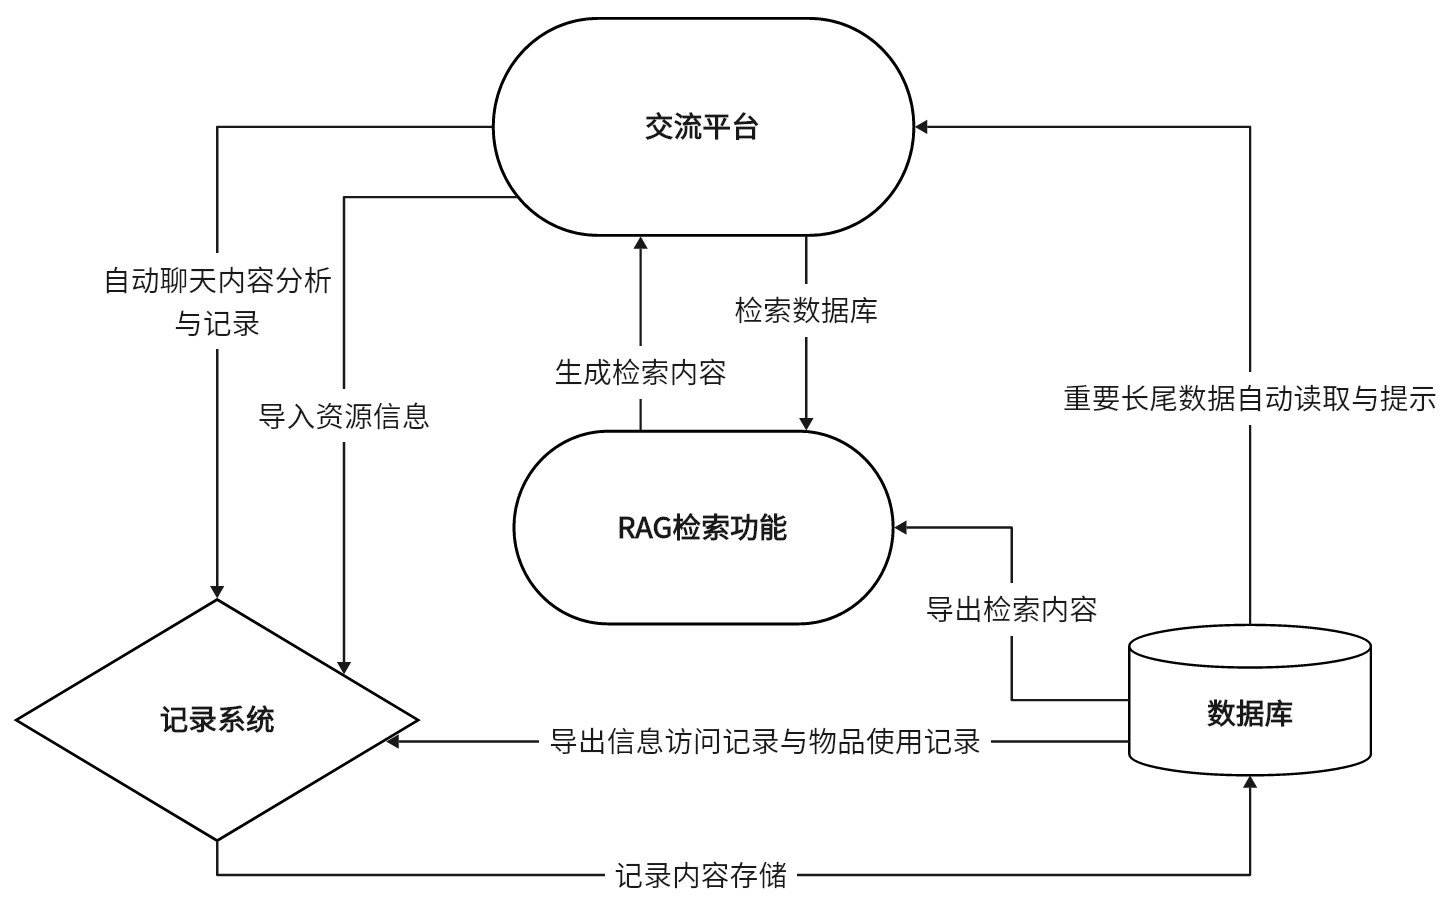
\includegraphics[width=0.9\textwidth]{系统整体.jpg} %插入图片,[]中设置图片大小,{}中是图片文件名
    \caption{系统整体构造示意} %最终文档中希望显示的图片标题
    \label{example_label} %用于文内引用的标签
\end{figure}
\subsection{系统各部分拆分详解}
 \subsubsection{记录系统}记录系统分为物品记录系统和数据记录系统。

\textbf{物品记录系统:}对于团队合作中用于共享的工具或仪器等物品,若存在产品说明书、产品介绍等内容,用户可直接通过交流平台将其录入共享资源库中并进行自动分析。
\begin{figure}[H]
	\centering
	\begin{subfigure}{0.8\textwidth}
		\centering
		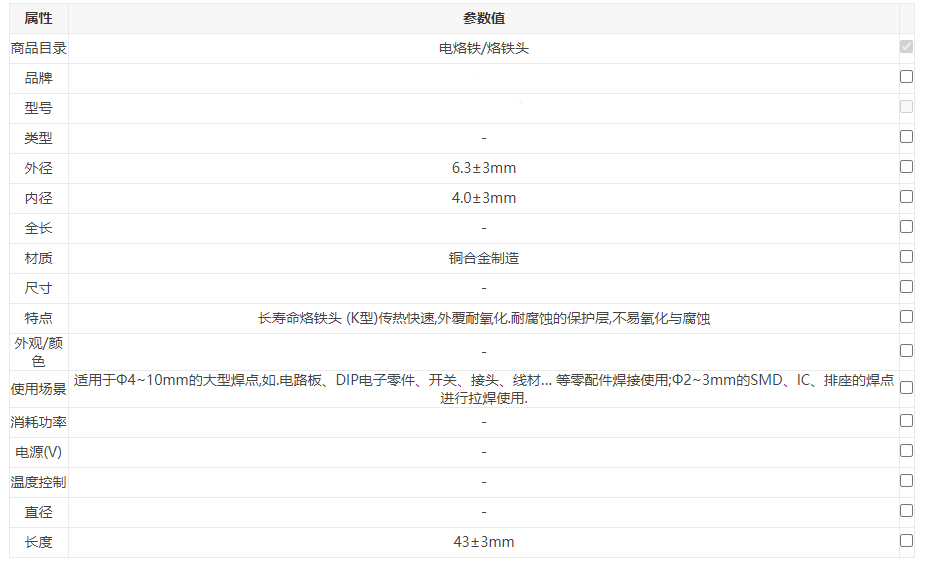
\includegraphics[width=0.9\textwidth]{电烙铁.png}
		\caption{某品牌电烙铁产品参数图}
		\label{chutian1}%文中引用该图片代号
	\end{subfigure}
	\qquad
	%让图片换行,
	\begin{subfigure}{0.8\linewidth}
		\centering
		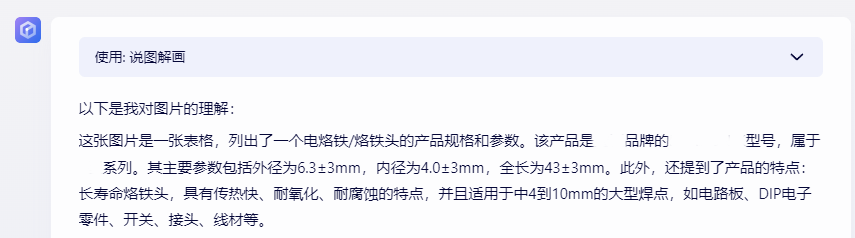
\includegraphics[width=0.9\linewidth]{文心一言.png}
		\caption{AI自动分析示例}
		\label{chutian2}%文中引用该图片代号
	\end{subfigure}
\caption{自动分析功能演示}
\label{qmix-train}
\end{figure}
完成自动分析之后,系统将自动生成对应物品名称、功能等内容。若系统发现存在信息缺失,将自动提示用户补充录入。
\begin{figure}[H] %H为当前位置,!htb为忽略美学标准,htbp为浮动图形
    \centering %图片居中
    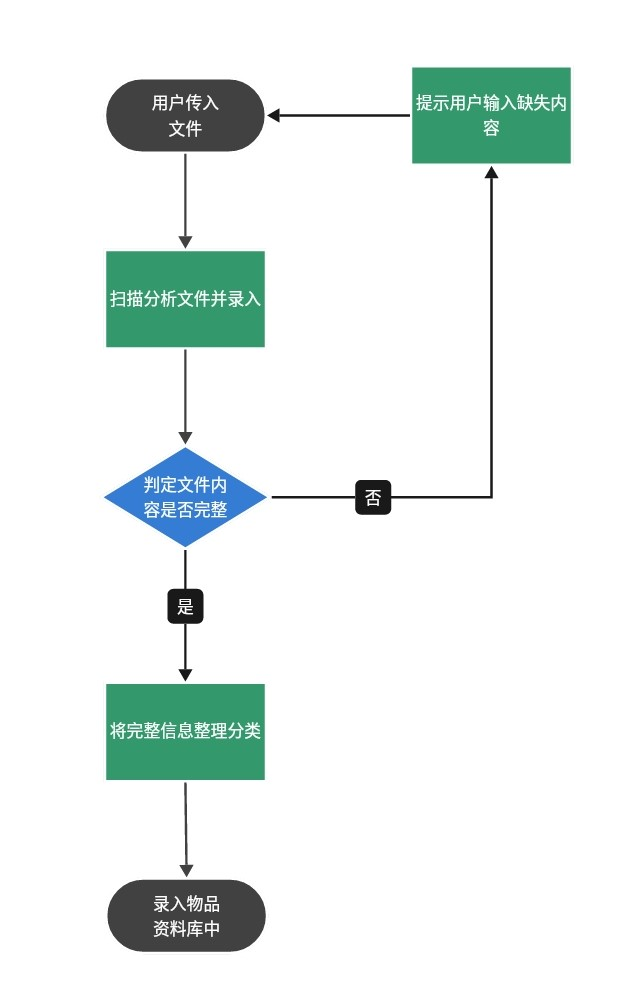
\includegraphics[width=0.6\textwidth]{物品信息导入.jpg} %插入图片,[]中设置图片大小,{}中是图片文件名
    \caption{物品导入流程} %最终文档中希望显示的图片标题
    \label{example_label} %用于文内引用的标签
\end{figure}
设想当中,一个较为完整的物品信息如表\ref{a}所示,若存在其他需要备注的内容,用户再根据实际应用过程中存储和使用情况使用本系统修改或添加信息即可。
\begin{table}[H]
\small
\caption{物品信息表及示例}
\centering
\begin{tabular}{cccccc}
\hline  
\textbf{名称} & \textbf{尺寸} & \textbf{使用场景} & \textbf{存放位置} & \textbf{使用情况} & \textbf{备注} \\ 
\hline  
电烙铁 & -  & 4-10mm大型焊点  & 成员A个人工具箱  & 未使用 & 加热速度较慢\\
\\
真空箱 & \makecell{内空间\\500*500*1000mm} & 真空实验 & 实验室北桌  & \makecell{使用中\\(成员A)} & -\\
\hline
\label{a}
\end{tabular} 
\end{table}

\textbf{数据记录系统:}信息记录系统主要功能为自动记录聊天记录、自动记录文件档案等,并应用大语言模型自动对其进行分析和纲要总结。除此之外,在设想之中,本系统还能够根据数据库内的信息生成各成员工作进度报告,并存储至数据库中。在具体应用过程中,有了新一代的大语言模型的嵌入,该系统应当能够承担信息收集、自动问题解答和处理、文本摘要和分析、自动化报告生成等职责\cite{7}。
\begin{table}[H]
\caption{数据信息表及示例}
\small
\centering
\begin{tabular}{ccccc}
\hline  
\textbf{编号} & \textbf{记录时间} & \textbf{信息内容} & \textbf{要点分析} & \textbf{备注} \\ 
\hline  
Chat-240320-1 & 3.20 & 聊天记录  & 四月日程、分工  & -\\
\\
File-240217-1&2.17&竞赛章程.pdf &竞赛内容、竞赛时间 & \makecell{已更新,请参考\\File-240301-1}\\
\hline
\label{b}
\end{tabular} 
\end{table}
 \subsubsection{交流平台 }本系统交流平台基本思路与传统沟通平台无太大差异,主要区别在于本交流平台在保留沟通交流和文件传输功能的同时将RAG检索功能嵌入其中。根据RAG模型已有的应用\cite{5}来看,相较于传统沟通平台而言,该模型的嵌入能够使其具备模糊内容检索、自动总结、自动答复功能。
\begin{figure}[H] %H为当前位置,!htb为忽略美学标准,htbp为浮动图形
    \centering %图片居中
    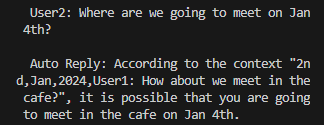
\includegraphics[width=0.6\textwidth]{自动答复示例.png} %插入图片,[]中设置图片大小,{}中是图片文件名
    \caption{自动答复功能示意} %最终文档中希望显示的图片标题
    \label{example_label} %用于文内引用的标签
\end{figure}
同时,在交流过程中提出的合作思路或分工,可以通过上文所述的记录系统将交流记录存储至共享资源库中,从而有助于后续具体合作流程的安排。
 \subsubsection{共享资源库 }
作为本系统运行的核心,共享资源库的设想借鉴了现代智能企业资产管理系统,并对其进行了轻量化和专业化修改。在应用RAG模型的基础上,数据库的修改和利用将变得更加便利化、智能化。在目前的设想中,该资源库主要分为四个部分,分别为管理团队内资源的物品资源库和信息资源库与管理团队外围资源的学术期刊库和新闻周边库。日后,用户可以根据具体的使用情况和需求自行增删数据库。
\begin{table}[H]
\small
\centering
\caption{共享资源库组成}
\begin{tabular}{|l||c|c|c|c|c|c|}
\hline
{\textbf{资源库名称}}     & \textbf{物品资源库} 	    &\textbf{信息资源库} 	  &\textbf{学术期刊库}     &\textbf{新闻周边库} 		\\ \hline
{\textbf{存储内容}} 		& 工具、仪器等			&研究思路、时间安排等		&各相关学术期刊等 	 &相关新闻等		\\ \hline
{\textbf{功能应用}}              &物品登记共享				&信息交流与公开		&思路借鉴与方法学习	   &修缮研究创新方案		\\ \hline
\end{tabular}
\end{table}
得益于记录系统,共享资源库的录入更加便利。对于管理团队内资源的库而言,用户可以应用上文所示的智能记录系统将内容录入库中,即可在接下来短期或长期的合作过程中持续方便使用;而对于管理团队外围资源的库来说,用户只需要提前选择好合作的研究或者创新大致方向,系统便能够根据对应方向的关键词检索功能从相关网站上筛选出对应内容并自动分类,然后录入库中。
\begin{figure}[H] %H为当前位置,!htb为忽略美学标准,htbp为浮动图形
    \centering %图片居中
    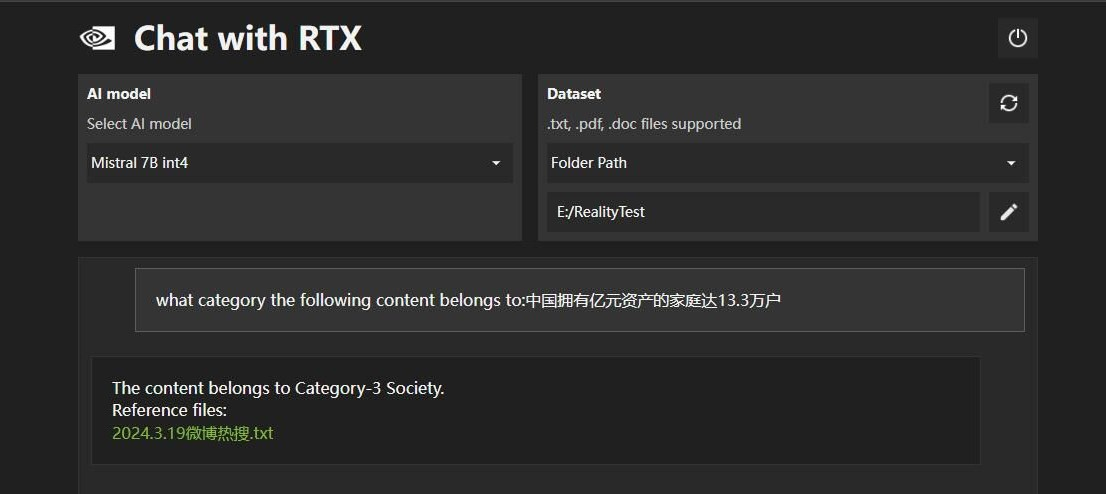
\includegraphics[width=0.8\textwidth]{自动分类示例.jpg} %插入图片,[]中设置图片大小,{}中是图片文件名
    \caption{应用Chat with RTX的RAG分类演示} %最终文档中希望显示的图片标题
    \label{example_label} %用于文内引用的标签
\end{figure}
RAG模型的应用将使得资源库的检索更加便利快捷。例如,可以通过搜索需求匹配对应物品、通过搜索应用对象和应用内容等匹配相关创意思路等。将RAG模型应用至资源库导致的更智能有效的检索能极大提高团队资源利用水平和利用效率。
\begin{figure}[H] %H为当前位置,!htb为忽略美学标准,htbp为浮动图形
    \centering %图片居中
    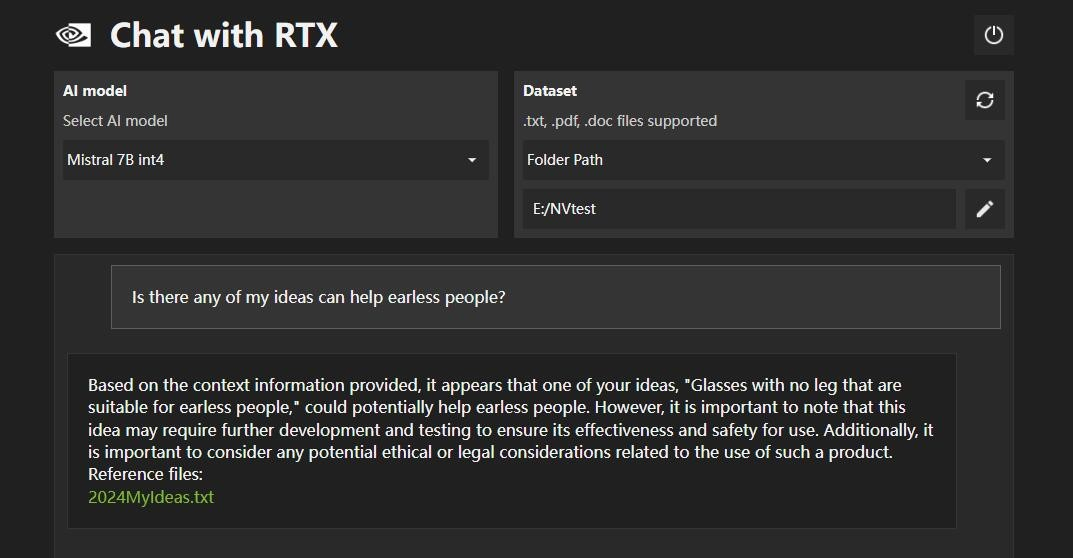
\includegraphics[width=0.8\textwidth]{RAG测试1.jpg} %插入图片,[]中设置图片大小,{}中是图片文件名
    \caption{应用Chat with RTX的RAG检索演示} %最终文档中希望显示的图片标题
    \label{example_label} %用于文内引用的标签
\end{figure}

  本系统的各个功能均已有对应开源软件可进行实现,而本系统主要是将这些功能进行整合串接,以求达到更有利地协助小型团队合作与团队内资源共享的目的。由此而言,本系统技术上是完全可行的。
\subsection{系统合理性分析}
\subsubsection{团队协作}
团队协作能力指建立在团队的基础之上,发挥团队精神、互补互助以达到团队最大工作效率的能力。团队协作能力包含人际沟通能力、责任感、团队合作精神和奉献精神等隐性因子\cite{6}。若从个人能力方面考量,团队协作能力的提高需要长年累月的学习才能够提升;但是在有恰当工具的辅助之下,团队协作水平便能够不再局限于团队成员本身的协作能力而产生质的变化。由于本系统聊天平台开发时借鉴了钉钉等针对于企业的人力协作系统,下文先引出企业提高人力资源利用率的模型:

为了有效整合和利用人力资源,企业需要遵循一个明确的三步流程模型。首先,要选择合适的平台,明确目标和制定规则,以确保群体的贡献能够得到有效聚合或过滤。其次,企业需要建立与群体的沟通渠道,提供必要的激励,并妥善处理知识产权保护和服务质量保障等挑战。最后,通过不断学习和优化协作策略,企业可以逐步提高自身的创新能力和竞争力\cite{8}。

由于企业本身就是基于小型组织和团队发展而来,相当于一个相较于小型团队拥有更加复杂的组织系统的大型团队,因此,企业对人力资源的利用方式在一定程度上可以移植至科研创新团队协作这一过程中。其一,本系统中记录系统与数据库的相互配合,对团队协作目标和分工、日程等规则与数据信息的自动记录和共享,能够确保群体的劳动成果的有效利用与整合;其二,沟通交流平台一方面保证了交流和成员激励的便利化,一方面为日后的成果划分等给出了详细的参考内容;其三,数据库的自动数据反馈能够协助团队优化合作方案与策略。
\subsubsection{资源共享}
Penrose 的著作首次提出将公司概念化为协调的资源束,以解决如何实现其目标和战略行为。他所关注的是,它创新性地将公司看成资源的集合公司可以对包括人力资源、实物资源等在内的异质资源进行高效获得和合理分配,这样可以帮助公司提高业绩,并进而形成与其他企业不同的竞争优势,进而推动自身稳定成长\cite{9}。对于小型科研创新团队而言,本系统为之提供了学术资源和社会信息资源更为便利的的获取,同时资源库的设立也能使其更合理分配现有资源。

综上所述,我们有充分的理由可以认为,虽然本系统目前只是存在于设想之中,但是在科研创新方面符合团队协作和资源共享的重大要求,具有其存在合理性与研发价值。
\section{本系统设想可能存在的问题与未来发展方向}
  一方面,由于本系统目前主要处于设想之中,因此面对实际应用情况可能将存在一定问题,这需要后续系统的完善与改进;另一方面,本系统在设计之初皆使用开源数据进行演示,因此针对特殊化的作业需要进行进一步的定制与修改。同时,针对团队中不同的使用身份,如领导者、策划者、设计者等,本系统目前并未做出相应规划,未来的发展中也需要进行针对身份的单独定制。
\section*{结论}% section*生成无标号章节
\addcontentsline{toc}{section}{结论} % 将无标号章节添加至目录
基于上述材料文本所描述的基于检索增强生成的协作与资源管理系统设想,我们可以预见,该系统在未来科研创新合作与资源利用最大化方面将发挥重要作用。通过应用大语言模型与检索增强生成技术,该系统能够有效地提升团队协作的效率和资源管理的智能化水平。

检索增强生成模型的引入,不仅可以通过结合检索与生成的能力,从大量知识库中精准选取和更新信息,进而提升系统生成内容的准确性和时效性;而且,该技术还有助于保护隐私数据,降低生成成本,并适用于跨模态和任务的应用场景。这些优势使得该系统在科研合作中能够更好地满足团队成员的信息需求,促进科研创新的深入开展。

综上所述,本系统具有广阔的应用前景和巨大的发展潜力。随着技术的不断进步和完善,该系统将在科研创新合作与资源利用方面发挥越来越重要的作用,为科研工作者提供更加便捷、高效的支持和服务。
\end{spacing}

\newpage

\addcontentsline{toc}{section}{参考文献} % 将无标号章节添加至目录
\begin{thebibliography}{99}
    \bibitem{1}简玮.企业资产数字化管理现状及有效对策研究[J].营销界,2023, (22). 
    \bibitem{2}韩熠星. 信息化时代医药集团企业固定资产管理问题分析 [J]. 西部财会,2022, (5).
    \bibitem{3}Patrick Lewis, Ethan Perez, Aleksandra Piktus. \textit{Retrieval-Augmented Generation for Knowledge-Intensive NLP Tasks}. NeurIPS 2020
    \bibitem{4}Vladimir Karpukhin, Barlas Oguz, Sewon Min, Ledell Wu, Sergey Edunov, Danqi Chen, and Wen-tau Yih. \textit{Dense passage retrieval for open-domain question answering}. arXiv: 2004.04906
    \bibitem{5}Penghao Zhao, Hailin Zhang, Qinhan Yu, Zhengren Wang, Yunteng Geng, Fangcheng Fu, Ling Yang, Wentao Zhang, Bin Cui.\textit{Retrieval-Augmented Generation for AI-Generated Content: A Survey}. arXiv: 2402.19473 
    \bibitem{7}李娜. 大语言模型在财务共享中心中的应用探究[J].中国农业会计,2024,34(06).
    \bibitem{6}何凤玲,王燕.影响中西方酒文化差异的因素[J].边疆经济与文化,2014(11).
    \bibitem{8}Prpic J.,Shukla P., Kietzmann J., McCarthy I., .\textit{How to work a
crowd:Developing crowd capital through crowdsourcing[J]}. Business Horizons,2015. 58(1):77-85.
 \bibitem{9} Wernerfelt B. \textit{A Resource-Based View of the Firm}[J]. Strategic Management Journal, 1984, (5):24-28
\end{thebibliography}
\bibliographystyle{gbt7714-numerical}

\end{document}
